\documentclass[review]{elsarticle}
% \usepackage[active, tightpage]{preview}

\usepackage{enumitem}
\usepackage{hyperref}
\usepackage{xcolor}
\hypersetup{
    colorlinks,
    linkcolor={red!50!black},
    citecolor={blue!50!black},
    urlcolor={blue!80!black},
    pdfborder={0 0 0}
}
\usepackage{multirow}
\usepackage{pgfplots}
\usepackage{float}
\usepackage{amssymb}
\usepackage{cleveref}
\usepackage[english]{babel}
\usepackage[utf8]{inputenc}
\usepackage[T1]{fontenc}
% \usepackage{changepage}
\usepackage{longtable}
\usepackage{tabularx}
\usepackage{pdfpages}
\usepackage{incgraph,tikz}
\usepackage[titles]{tocloft}
\setlength{\cftbeforesecskip}{-.5ex}
\renewcommand{\cftsecleader}{\cftdotfill{\cftdotsep}}

% \usepackage[showframe=true]{geometry}
%
\newcommand{\textttt}[1] {\texttt{\footnotesize#1}}
\newcommand{\h} {\hphantom ~ }
% \newcommand{\textttt}[1] {\mbox{\texttt{\footnotesize#1}}}
% \newcommand{\textttt}[1] {
% \begin{verbatim} #1 \end{verbatim}
% }
\pgfplotsset{compat=1.5}
\pgfplotsset
{
	width=0.5\textwidth,
	x tick label style={/pgf/number format/1000 sep=},
  enlarge x limits = 0.0,
  ymajorgrids=true,
	major tick style={draw=none},
  ymin = 0.0,
	every axis/.append style={
		every x tick label/.append style={font=\tiny},
    every y tick label/.append style={font=\tiny},
    every axis label/.append style={font=\small},
    height=37mm,
    width=37mm,
    title style={at={(0.5,0.90)}, font=\normalfont},
    xticklabel style={yshift=4pt}
	}
}

%% `Elsevier LaTeX' style
\bibliographystyle{elsarticle-num}
%
\makeatletter
\def\ps@pprintTitle{%
    \let\@oddhead\@empty
    \let\@evenhead\@empty
    \def\@oddfoot{}%
\let\@evenfoot\@oddfoot}
\makeatother
\begin{document}
%
\begin{frontmatter}
%
\title{Linked Open Social Data for Scientific Benchmarking (Supporting
Information document)}
%
\author[pwr]{Renato Fabbri\corref{corresponding}\fnref{kio-url}}
\ead{fabbri@usp.br}
%
\author[pwr]{Osvaldo Novais de Oliveira Junior\fnref{kio-url}}
\ead{chu@ifsc.usp.br}
%
\cortext[corresponding]{Corresponding author}
\address[pwr]{S\~ao Carlos Institute of Physics, S\~ao Paulo
University, Brazil}
%
\fntext[kio-url]{\textit{URL:} \url{http://www.ifsc.usp.br/}}
%
\begin{abstract}
This is a Supporting Information document which exposes ontological
diagrams and auxiliary tables for the Linked Open Social Data (LOSD)
database. The main document of the article is in~\cite{losd}.
\end{abstract}
%
\begin{keyword}
Big Data, Data Mining, Benchmark Data, Facebook, Twitter, IRC, Email,
Complex Networks, Text Mining
%Hierarchy of Clusters \sep HoC \sep Benchmark Dataset \sep Benchmark Data Generator \sep Artificial Data \sep Cluster Analysis \sep Tree Structured Stick Breaking Process \sep TSSB \sep ...
\end{keyword}

\end{frontmatter}
\newcommand{\foo}{\textheight}
\newcommand{\foobar}{\pdfpageheight}
% \pdfpageheight 8in
\tableofcontents
\clearpage
\section{General guidance}
% \paperheight = 200pt
In this document we provide diagrams
for the provenances in the LOSD:
Facebook, Twitter, IRC, Email, ParticipaBR, Cidade Democrática and AA.
Each provenance diagram was broken in two, one presents the relations
among main classes (blue nodes) and data types (orange nodes), the other presents metadata on the
snapshot.
Every class instance is related to the snapshot instance
by the triple \textttt{class\_uri po:snapshot snapshot\_uri}.
Such triples are omitted for simplicity.
Due to the large number of relations, the rendering of diagrams are
automatized and displays some overlaps.
Even so, the images are useful for grasping what is in current LOSD
and for conducting explorations.
Edges in the diagrams have:
\begin{itemize}
    \item green color if representing an OWL existential
class restriction (all individuals from the class present at least one triple with
the property as predicate);
    \item inverted nip if representing an OWL universal class
        restriction (all individuals presenting triples with the
        property as predicate are from the class);
    \item full edges (non-dashed) if representing a functional property
        axiom (there is at most one triple with the property as the
        predicate for each individual).
\end{itemize}

% \textheight = 100pt
% \pdfpageheight 300pt
Furthermore, this document ends with two sets of tables, one with counts of
triples, participants, edges/interactions/relations and characters,
the other with references for snapshot groups, such as wikipedia or
contact links.


\section{Facebook data}
Each Facebook snapshot is yield by either an user, from which the
friends constitute a friendship network, or a group, which participants
can yield friendship and interaction networks and posts information with
text and some metadata.
Further information is found on the following diagrams, the tables on
the end of this document or in the main document of this
article~\cite{losd}.

% 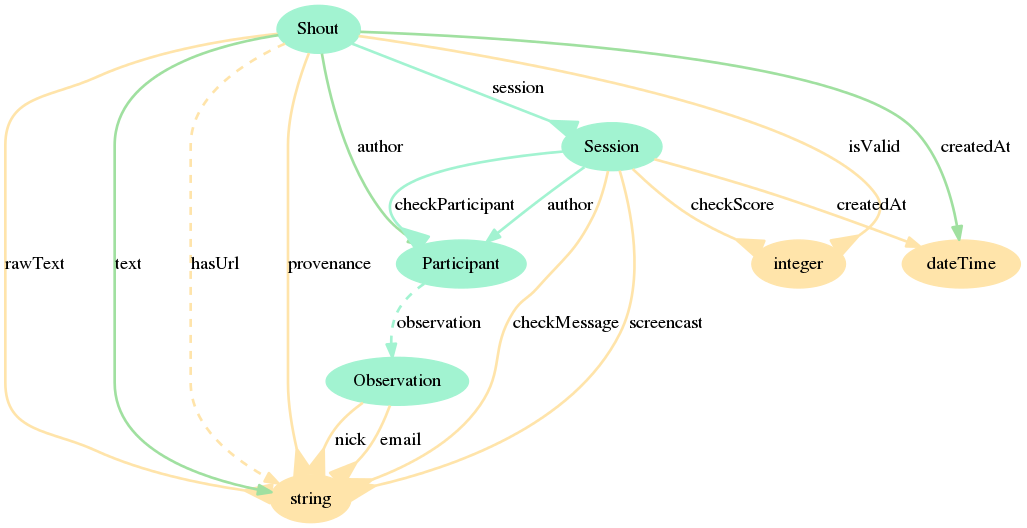
\includepdf{ontologies/aairc.ttl/draw.pdf}
\incgraph[
  overlay={\node[red,below right] at (page.north west) {\Huge Facebook};}
    paper=graphics
][scale=.6]{ontologies/facebook-legacy-Auricultura10042013Friendship.ttl/draw.png}

\textheight = 2in
\pdfpageheight 5in
\incgraph[
  overlay={\node[red,below right] at (page.north west) {\Huge Facebook};}
    paper=graphics
][scale=.5]{ontologies/facebook-legacy-Auricultura10042013Meta.ttl/draw.png}

\section{Twitter data}
Each Twitter snapshot is yield by a hashtag.
Retweets (\textttt{po:retweetOf} are usually considered to yield the interactions between users.
Users are identified through authors \textttt{po:numericID} (global as given by Twitter API)
or \textttt{}.
The database present also \textttt{po:replyTo} and \textttt{po:userMention}
which might also be useful in understanding the networking.
Further information is found on the following diagrams, the tables on
the end of this document or in the main document of this
article~\cite{losd}.

\incgraph[
  overlay={\node[red,below right] at (page.north west) {\Huge
  Twitter };}
    paper=graphics
][scale=.5]{ontologies/twitter-legacy-arenaNETmundialTweet00000.ttl/draw.png}

\incgraph[
  overlay={\node[red,below right] at (page.north west) {\Huge Twitter};}
    paper=graphics
][scale=.7]{ontologies/twitter-legacy-arenaNETmundialMeta.ttl/draw.png}

\section{IRC data}
Each IRC snapshot is yield by an IRC channel.
IRC messages are either server messages (e.g. join and exit channel)
marked with \textttt{po:systemMessage true} and having an \textttt{po:impliedUser user\_uri},
or user messages, which yield interactions through \textttt{po:directedTo} and \textttt{po:mentions} properties.
Text messages without the user names are delivered through the \textttt{po:cleanText} property.
Further information is found on the following diagrams, the tables on
the end of this document or in the main document of this
article~\cite{losd}.
\incgraph[
  overlay={\node[red,below right] at (page.north west) {\Huge IRC};}
    paper=graphics
][scale=.7]{ontologies/irc-legacy-hackerspace-cpsLog00000.ttl/draw.png}
\incgraph[
  overlay={\node[red,below right] at (page.north west) {\Huge IRC};}
    paper=graphics
][scale=.6]{ontologies/irc-legacy-hackerspace-cpsMeta.ttl/draw.png}

\section{Email data}
Each IRC snapshot is yield by an Email list.
Interactions is yield through \textttt{po:replyTo} relations
although \textttt{po:to} and \textttt{po:cc} can also be considered.
the email body is given by \textttt{po:text} relations while
\textttt{po:cleanText} has the text with lines removed where they are
trivially from previous messages or computer code.
Further information is found on the following diagrams, the tables on
the end of this document or in the main document of this
article~\cite{losd}.
\incgraph[
  overlay={\node[red,below right] at (page.north west) {\Huge Email};}
    paper=graphics
][scale=.4]{ontologies/gmane-legacy-linux.audio.devel1-20000Email00000.ttl/draw.png}
\textheight = 3in
\pdfpageheight 6in
\incgraph[
  overlay={\node[red,below right] at (page.north west) {\Huge Email};}
    paper=graphics
][scale=.5]{ontologies/gmane-legacy-linux.audio.devel1-20000Meta.ttl/draw.png}

\section{ParticipaBR data}
The ParticipaBR snapshot is yield by a data dump donated by the system
administrators of the federal portal of social participation ParticipaBR.
Articles can have parent articles (\textttt{po:parent}), be step of a
collection of articles (\textttt{po:stepOf}) and be a mediation of other
articles (\textttt{po:mediationOf}).
Interactions are yield by comments which are \textttt{po:replyTo} other
comments or which are made directly to an article.
This snapshot holds also friendship structures.
The language used is mainly Brazilian Portuguese, but English and
Spanish are also incident.
Due to the higher complexity of the diagram, an additional figure is
given rendered with another layout algorithm
Further information is found on the following diagrams, the tables on
the end of this document or in the main document of this
article~\cite{losd}.
\incgraph[
  overlay={\node[red,below right] at (page.north west) {\Huge
  ParticipaBR};}
    paper=graphics
][scale=.5]{ontologies/participabr.ttl/draw.png}
\incgraph[
  overlay={\node[red,below right] at (page.north west) {\Huge
  ParticipaBR};}
    paper=graphics
][scale=.7]{ontologies/participabr.ttl/draw_circo.png}
\incgraph[
  overlay={\node[red,below right] at (page.north west) {\Huge
  ParticipaBR};}
    paper=graphics
][scale=.7]{ontologies/participabrMeta.ttl/draw.png}

\section{Cidade Democrática data}
The Cidade Democrática snapshot is yield by a data dump donated by the system
administrators of the civil society social participation portal Cidade
Democrática.
This snapshot holds a complex structure of both
Topics/Inspirations/
Observatories/Supports/Competitions/Prizes
and of State/City/Neighborhood/Place.
The language used is mainly Brazilian Portuguese.
Due to the higher complexity of the diagram, an additional figure is
given rendered with another layout algorithm
Further information is found on the following diagrams, the tables on
the end of this document or in the main document of this
article~\cite{losd}.
\incgraph[
  overlay={\node[red,below right] at (page.north west) {\Huge Cidade
  Democrática};}
    paper=graphics
][scale=.4]{ontologies/cidadedemocratica00000.ttl/draw.png}
\textheight = 2in
\pdfpageheight 5in
\incgraph[
  overlay={\node[red,below right] at (page.north west) {\Huge Cidade
  Democrática};}
    paper=graphics
][scale=.4]{ontologies/cidadedemocratica00000.ttl/draw_circo.png}

\incgraph[
  overlay={\node[red,below right] at (page.north west) {\Huge Cidade
  Democrática};}
    paper=graphics
][scale=.7]{ontologies/cidadedemocraticaMeta.ttl/draw.png}

\section{AA data}
The AA (Algorithmic Autoregulation) snapshots are yield by a data dump donated by the system
administrators and by a mined IRC log.
The system pursue simplicity and most of data consists of detached
shouts with \textttt{po:text} and \textttt{po:author}.
Further information is found on the following diagrams, the tables on
the end of this document or in the main document of this
article~\cite{losd}.
\incgraph[
  overlay={\node[red,below right] at (page.north west) {\Huge AA};}
    paper=graphics
][scale=.6]{ontologies/aairc.ttl/draw.png}
\textheight = 7in
\pdfpageheight \foobar
\incgraph[
  overlay={\node[red,below right] at (page.north west) {\Huge AA};}
    paper=graphics
][scale=.7]{ontologies/aaircMeta.ttl/draw.png}

\section{Snapshot references}
\label{sreferences}
\pdfpageheight 10in
All the Facebook snapshots are either the result of individuals who downloaded
their data (and donated to the first author) or data downloaded from groups.
In the first case, it is senseless to present references and the. In the second
case, we present the group name and a link to a post in the group where
data and figures were delivered to the group.



\begin{table*}[h!]\scriptsize
\begin{center}
\caption{Different Twitter snapshots are yield by different hashtags. In this
table we present each snapshot with the respective hashtag and a
reference to the subject.}\label{tab:provenance}
\begin{tabular}{| l || p{4cm} | p{4cm} | }\hline
    \textbf{snapshot hashtag} & \textbf{observation} & \textbf{reference} \\\hline\hline
    \#arenaNETmundial & a Brazilian discussion hub about free culture, democracy and the internet & \url{http://www.participa.br/netmundial} \\\hline
    \#art & tweets with the generic hashtag \#art & \url{https://en.wikipedia.org/wiki/Art} \\\hline
    \#ChennaiFloods & heavy rainfall generated by the annual northeast monsoon in November–December 2015 & \url{https://en.wikipedia.org/wiki/2015_South_Indian_floods} \\\hline
    \#dilma & the 36th President of Brazil & \url{https://en.wikipedia.org/wiki/Dilma_Rousseff} \\\hline
    \#ForaDilma & 2015-16 anti-government protests in Brazil & \url{https://en.wikipedia.org/wiki/2015-16_protests_in_Brazil} \\\hline
    \#ForaCunha & 2015-16 anti-corruption protests in Brazil & \url{https://en.wikipedia.org/wiki/2015-16_protests_in_Brazil} \\\hline
    \#fuck & tweets with the generic hashtag \#fuck & \url{https://en.wikipedia.org/wiki/Fuck} \\\hline
    \#game & tweets with the generic hashtag \#game & \url{https://en.wikipedia.org/wiki/Game} \\\hline
    \#god & tweets with the generic hashtag \#god & \url{https://en.wikipedia.org/wiki/God} \\\hline
    \#MAMA2015 & the grand 2015 Mnet Asian Music Awards & \url{https://en.wikipedia.org/wiki/2015_Mnet_Asian_Music_Awards} \\\hline
    \#music & tweets with the generic hashtag \#music & \url{https://en.wikipedia.org/wiki/Music} \\\hline
    \#obama & the 44th President of the United States & \url{https://en.wikipedia.org/wiki/Barack_Obama} \\\hline
    \#python & the Python programming language & \url{https://en.wikipedia.org/wiki/Python_(programming_language)} \\\hline
    \#QuartaSemRacismoClubeSDV & an anti-racism netweaving & \url{https://twitter.com/hashtag/quartasemracismoclubesdv} \\\hline
    \#science & tweets with the generic hashtag \#science & \url{https://en.wikipedia.org/wiki/Science} \\\hline
    \#SnapDetremura & reference for Snapchat about a celebrated person & \url{https://twitter.com/detremura} \\\hline
\end{tabular}\end{center}
\end{table*}                    


\begin{table*}[h!]\scriptsize
\begin{center}
\caption{Different IRC snapshots are yield by different channels. In this
table we present each snapshot with the respective channel and a
reference to the subject.}\label{tab:provenance}
\begin{tabular}{| l || p{4cm} | p{4cm} | }\hline
    \textbf{snapshot channel} & \textbf{observation} & \textbf{reference} \\\hline\hline
    \#foradoeixo & a Brazilian network of culture related collectives & \url{https://pt.wikipedia.org/wiki/Fora_do_Eixo} \\\hline
    \#hackerspace-cps & a hackerspace in Campinas, Brazil & \url{https://lhc.net.br/wiki/P%C3%A1gina_principal} \\\hline
    \#hackerspaces-br & Brazilian hackerspaces channel & \url{https://garoa.net.br/wiki/Hackerspaces_Brasileiros} \\\hline
    \#labmacambira & Brazilian channel for the labMacambira collective & \url{http://labmacambira.sourceforge.net/} \\\hline
\end{tabular}\end{center}
\end{table*}                    

\begin{table*}[h!]\scriptsize
\begin{center}
\caption{Different Email snapshots are yield by different email lists. In this
table we present each snapshot with the respective list and a
reference to the subject.}\label{tab:provenance}
\begin{tabular}{| l || p{4cm} | p{4cm} | }\hline
    \textbf{Gmane ID} & \textbf{observation} & \textbf{reference} \\\hline\hline
    gmane.linux.audio.users & the Linux Audio Users & \url{http://linuxaudio.org} \\\hline
    gmane.politics.organizations.metareciclagem & a network about technology and social transformation  & \url{https://metareciclagem.github.io} \\\hline
    gmane.linux.audio.devel & the Linux Audio Developers & \url{http://lists.linuxaudio.org/listinfo/linux-audio-dev} \\\hline
    gmane.comp.gcc.libstdc++.devel & the C++ standard library & \url{https://gcc.gnu.org/libstdc++/} \\\hline
\end{tabular}\end{center}
\end{table*}                    
 
\begin{table*}[h!]\scriptsize
\begin{center}
\caption{References for the snapshots of the detached instances
ParticipaBR, Cidade Democrática and AA.}\label{tab:provenance}
\begin{tabular}{| l || p{4cm} | p{3cm} | }\hline
    \textbf{social protocol} & \textbf{observations} & \textbf{reference} \\\hline\hline
    ParticipaBR & a Brazilian federal portal of social participation & \url{http://www.participa.br/} \\\hline
    Cidade Demorática & a Brazilian civil society portal of social participation & \url{http://www.cidadedemocratica.org.br/} \\\hline
    AA & the Algorithmic Autoregulation software development methodology & \cite{aarticle} \\\hline
\end{tabular}\end{center}
\end{table*}                    








\clearpage


\section*{References}

%
\bibliography{paper}
%\bibliography{myLastBibfile.bib}
%
\end{document} 
